\section{Tutorial - ADC Metrics}

\subsection{Leanring Objective}

By the end of this practical, you will have:
\begin{itemize}
    \item Practical understanding of ADC metrics and how this should help you quantify the performance of an ADC or DAC device; and
    \item Simple practical experience of using data sampled from an ADC in order to find ADC metrics.
\end{itemize}

\textit{Preparatory notes:} For this tutorial, it is assumed you know the basics of sampling; if you feel a bit shaky on this theory, then read over Lecture 27 slides 6 - 21.

\subsection{ADC Metrics}

Consider the following scenario and then respond to the questions that follow.

\textbf{Scenario:}

Consider that you’re in lockdown. You and your colleague are working remotely to implement sampling in the system you are tasked do build. As it happens neither of you have access to the physical platform, but being a smart engineer you hooked it up to the internet as well as a remotely controlled signal generator and remote-controlled power switch before abandoning the office. So you both have access to the platform, which happens to be running embedded Linux and is connected via ssh. 

What you do know is that it’s an 8-bit ADC. It’s a low-cost SPI ADC that isn’t of the best quality. You can assume that you’ve got the code to program it. 

But you need to answer a few questions in order to decide on processing solutions to implement. Various data files have been obtained from tests that were run which will help you to characterize the ADC. The ADC is set up to receive a 0 – 2.55V signal, to convert that to a 8-bit values. The ADC is sampling at 1MHz. It understandably has a DC offset of some sort and saturates at some point.

\subsubsection{Question 1}

First off, the most obvious thing first: we know it’s an 8-bit ADC but that doesn’t mean it gives that perfect resolution. Considering that a ramp waveform has been linked up to test things. The ramp is running at 250KHz, and we sample for 10K (as in 10*1024) samples (each sample being 1us, so do the math to see how long the sample block is, if you want to know that).
We’ve set up the voltage range to go from 0 to 2.50V also. But we also already know the device saturates at some point below 2.55V, thus setting the signal generator’s maximum voltage above 2.5V wouldn't make sense.

The captured data file is stored in \href{http://ocw.ee.uct.ac.za/courses/EEE3096S/miscres/adcmet1/ramp.csv}{ramp.csv} and shown in figure \ref{fig:ramp} below. Investigate the file and determine the answer to the following sub-questions:

\begin{enumerate}
\item What is the resolution in bits of the ADC? Based on the samples obtained from the experiment? [5 marks]
\item What is the Q (Quantizing) Resolution in Volts for this system?  (i.e. do some inspections to determine the difference between two input voltages causing the digitized output to be incremented by 1). [5 marks]
\end{enumerate}

Provide clear explanations (or working) for both your above answers.

\begin{figure}[H]
\centering
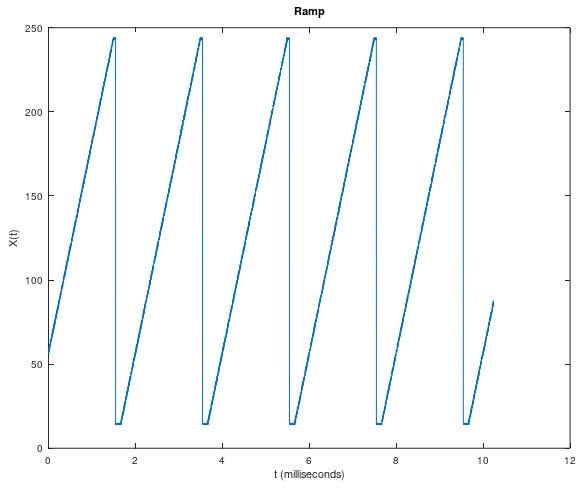
\includegraphics[width=0.8\columnwidth]{Body/ADC_Voltmeter/images/eee_adcmet_pr01_ramp.jpg}
\caption{Testing of feeding a ramp into the ADC, ramp.csv sample file}
\label{fig:ramp}
\end{figure}

\subsubsection{Question 2}

For this case, we have fed 0V into the ADC (or as good at the remote-controlled signal generator, that is connected to the platform, can do 0V; which is pretty good). The 10K sample recording is provided in \href{http://ocw.ee.uct.ac.za/courses/EEE3096S/miscres/adcmet1/zero.csv}{zero.csv}. You can see it’s not exactly zero or perfectly behaved. Basically it is not getting down to 0V. Answer the following based on this recording:

\begin{enumerate}
\item What is the direct current (DC) offset error of the ADC when it is conncted to OV? [5 marks]
\item A further test was done in which the signal generator was told to generate a frequency of 80KHz, for which we got another 10K samples. The recorded data is provided at \href{http://ocw.ee.uct.ac.za/courses/EEE3096S/miscres/adcmet1/freq1.csv}{freq1.csv}. The frequency plot generated from an FFT is shown in figure \ref{fig:freq1}. Use this data determine what the Spurious-free Dynamic Range (SFDR). Provide you answer as either power or S/N (or both if you want to be fancy). Note: you need to show your working, you can include a snippet of figures of your working to motivate your answer. As you have probably noticed, there is another signal picked up, assume this is an aliased 50Hz and basically something that one has to live with when using this device. [10 marks]
\end{enumerate}

\begin{figure}[H]
\centering
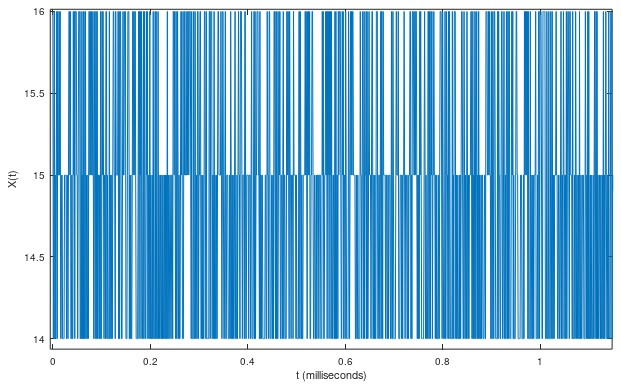
\includegraphics[width=0.8\columnwidth]{Body/ADC_Voltmeter/images/eee_adcmet_pr01_zero.jpg}
\caption{Testing at 0V input, a zoomed in view of the zero.csv captured data}
\label{fig:zerosamp}
\end{figure}

\begin{figure}[H]
\centering
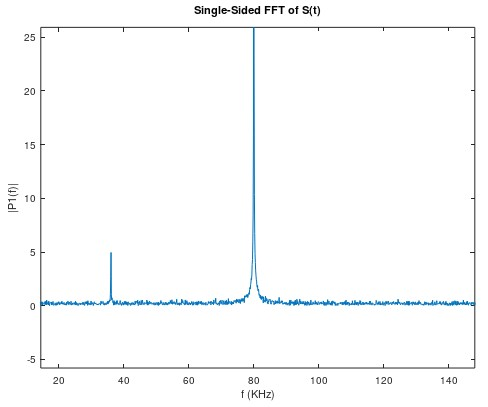
\includegraphics[width=0.8\columnwidth]{Body/ADC_Voltmeter/images/eee_adcmet_pr01_freq1.jpg}
\caption{Testing with 80KHz input, a zoomed in view of frequency plot}
\label{fig:freq1}
\end{figure}

